\documentclass[10pt]{article}
\usepackage[utf8]{inputenc}
\usepackage[italian]{babel}
\usepackage{multicol}
\usepackage[bookmarks]{hyperref}
\usepackage[a4paper, total={18cm, 25cm}]{geometry}
\usepackage{listings}
\usepackage{graphicx}
\usepackage{makecell}
\graphicspath{ {./img/} }
\usepackage{color}
\definecolor{mygray}{rgb}{0.5,0.5,0.5}
\usepackage{listings}
\usepackage{qtree}
\lstset{
	language=SQL,
	breaklines=true,
	keywordstyle=\bfseries,
	identifierstyle=\ttfamily,
	commentstyle=\color{mygray},
	morekeywords={database, REFERENCES, SCHEMA, AUTHORIZATION, PROCEDURE, WITH, CHECK, OPTION, FOR, EACH, ROW, DECLARE, BEFORE, AFTER, IF, TO, PRIVILEDGES, COMMIT, WORK, ROLLBACK, SORT},
}

\begin{document}
\renewcommand*\contentsname{Indice}
\title{Corso di Basi di Dati A.A. 2019/20\\Progetto BD VIII}
\author{Federico Matteoni\\Mat. 530257}
\date{24/03/2021}
\maketitle
\pagebreak
\section{Descrizione del dominio}
Uno studio professionale vuole tenere traccia delle pratiche in corso.\\\\
Si vuole tenere traccia dei clienti, che possono essere persone o organizzazioni.\\
Di ogni cliente, ci interessano il nome, l'indirizzo ed un recapito telefonico.\\
Delle persone, ci interessano anche il cognome ed il codice fiscale.\\ Delle organizzazioni ci interessa anche la partita IVA e quali persone svolgono un ruolo al suo interno, ed il ruolo svolto.\\\\
Si vuole tenere traccia delle pratiche, di cui un cliente è titolare.\\
Se il titolare è un'organizzazione, ci interessa sapere le persone che seguono tale pratica.\\\\
Si emettono fatture intestate ad un cliente e relative ad una pratica.\\\\
I clienti effettuano pagamenti, totali o parziali, legati ad una o più fatture e di cui ci interessa sapere la modalità con cui sono stati eseguiti.
\section{Schema Concettuale}
\begin{center}
	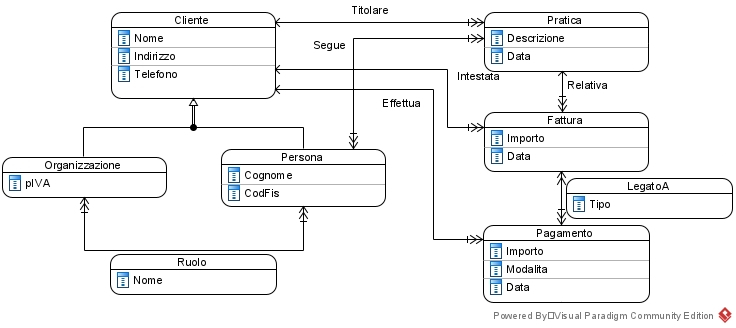
\includegraphics[scale=0.9]{Concettuale.jpg}
\end{center}
\section{Schema Logico Relazionale}
\begin{center}
	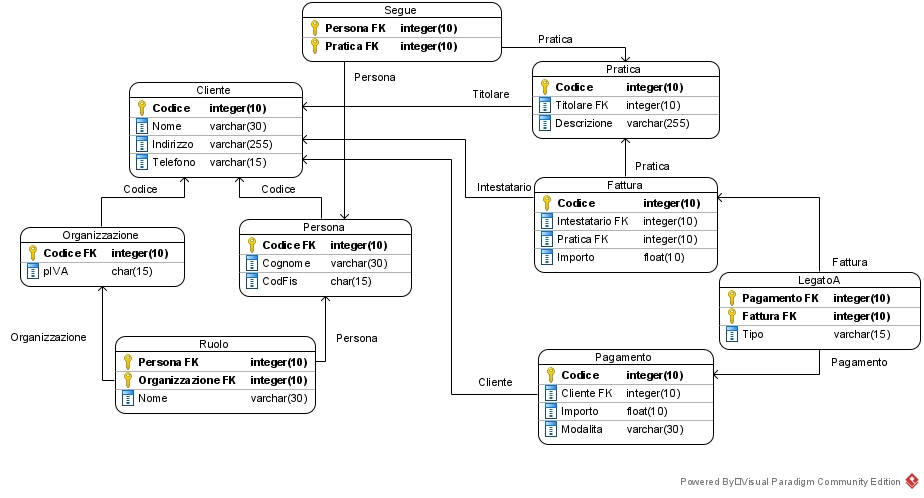
\includegraphics[scale=0.5]{LogicoRelazionale.jpg}
\end{center}
\begin{list}{}{\textbf{Notazione testuale}}
	\item Cliente(\underline{Codice}, Nome, Indirizzo, Telefono)
	\item Organizzazione(\underline{Codice*}, pIVA)
	\item Persona(\underline{Codice*}, Cognome, CodFis)
	\item Ruolo(\underline{Persona*}, \underline{Organizzazione*}, Nome)
	\item Pratica(\underline{Codice}, Titolare*, Descrizione, Data)
	\item Segue(\underline{Persona*}, \underline{Pratica*})
	\item Fattura(\underline{Codice}, Intestatario*, Pratica*, Importo, Data)
	\item Pagamento(\underline{Codice}, Cliente*, Importo, Modalità, Data)
	\item LegatoA(\underline{Pagamento*}, \underline{Fattura*}, Tipo)
\end{list}
\begin{list}{}{\textbf{Vincoli non catturati graficamente}}
	\item $\forall$ tupla $s\:\in$ Segue e per la tupla $p\:\in$ Pratica associata, si ha che $\exists$ tupla $r\:\in$ Ruolo con $s$[Persona] = $r$[Persona] $\wedge$ $p$[Titolare] = $r$[Organizzazione]\\
	Cioè ogni persona che segue una pratica ha un ruolo nell'organizzazione titolare di tale pratica.
\end{list}
\pagebreak
\section{Query SQL}
\begin{enumerate}
	\item Uso di proiezione, join e restrizione\\
	La lista dei clienti con pagamenti superiori a 1000 euro.
	\begin{lstlisting}
	SELECT Nome
	FROM Cliente JOIN Pagamento ON Cliente.Codice = Pagamento.Cliente
	WHERE Importo > 1000
	\end{lstlisting}
	\item Uso di group by con having, where e sort\\
	La classifica delle modalità di pagamento per somma d'importi, per somme maggiori di 1000 euro e singoli pagamenti maggiori di 500 euro.
	\begin{lstlisting}
	SELECT Modalita, SUM(Importo) AS Totale
	FROM Pagamento
	WHERE Importo > 500
	GROUP BY Modalita
	HAVING Totale > 1000
	ORDER BY Totale
	\end{lstlisting}
	\item Uso di join, group by con having e where\\
	La lista delle fatture con più di 10 pagamenti inferiori ai 500 euro.
	\begin{lstlisting}
	SELECT Fattura, COUNT(LegatoA.Pagamento) AS Pagamenti
	FROM LegatoA JOIN Pagamento ON LegatoA.Pagamento = Pagamento.Codice
	WHERE Importo < 500
	GROUP BY LegatoA.Fattura
	HAVING Pagamenti > 10
	\end{lstlisting}
	\item Uso di select annidata con quantificazione esistenziale\\
	Le persone che hanno almeno un ruolo in un'organizzazione.
	\begin{lstlisting}
	SELECT Codice
	FROM Persona
	WHERE EXISTS (SELECT * FROM Ruolo WHERE Ruolo.Persona = Persona.Codice)
	\end{lstlisting}
	\item Uso di select annidata con quantificazione universale\\
	Le persone che non seguono alcuna pratica.
	\begin{lstlisting}
	SELECT Codice
	FROM Persona
	WHERE Codice NOT IN (SELECT Persona FROM Segue)
	\end{lstlisting}
	\item Uso di subquery di confronto quantificato usando una subquery\\
	I pagamenti superiori alla media.
	\begin{lstlisting}
	SELECT *
	FROM Pagamento
	WHERE Importo > (SELECT AVG(Importo) FROM Pagamento)
	\end{lstlisting}
\end{enumerate}
\pagebreak
\section{Piani di accesso}
\begin{enumerate}
	\item Scrivere un piano di accesso logico delle query 1, 2 e 3 abbreviati con le iniziali.
	\begin{list}{}{}
		\item[1.]		
\Tree [.$\pi$\\Nome [.$\sigma$\\Importo$\:>\:$1000 [.$\bowtie$\\Cliente.Codice$\:$=$\:$Pagamento.Cliente  Cliente Pagamento ] ] ]\\\\
		\item[2.]		
		\Tree [.$\tau$\\Totale [.$\pi$\\Modalita,$\:$Totale [.$\sigma$\\Totale$\:>\:$1000 [.$\rho$\\SUM(Importo)$\leftarrow$Totale [.Modalita$\:\gamma\:$SUM(Importo) [.$\sigma$\\Importo$\:>\:$500 Pagamento ] ] ] ] ] ]\\\\
		\item[3.]		
		\Tree [.$\pi$\\Fattura,$\:$Pagamenti [.$\sigma$\\Pagamenti$\:>\:$10 [.$\rho$\\COUNT(LegatoA.Pagamento)$\leftarrow$Pagamenti [.Fattura$\:\gamma\:$COUNT(LegatoA.Pagamento) [.$\sigma$\\Importo$\:<\:$500 [.$\bowtie$\\LegatoA.Pagamento$\:$=$\:$Pagamento.Codice LegatoA Pagamento ] ] ] ] ] ]
	\end{list}
	\pagebreak
	\item Scrivere un piano di accesso fisico efficiente per i tre piani di accesso logico al punto 1 che non fanno uso di indici e (opzionale) verificare se la sort prima della group by può essere evitata.\\\\
		1.
		\Tree [.Project(\{Nome\}) [.Filter(Importo$\:>\:$1000) [.NestedLoop(Cliente.Codice$\:$=$\:$Pagamento.Cliente)  TableScan(Cliente) TableScan(Pagamento) ] ] ]\\\\\\
		2.
		\Tree [.Sort(\{SUM(Importo)\}) [.Project(\{Modalita,$\:$SUM(Importo)\}) [.Filter(SUM(Importo)$\:>\:$1000) [.GroupBy(\{Modalita\},$\:$\{SUM(Importo)\}) [.Filter(Importo$\:>\:$500) SortScan(Pagamento,$\:$\{Modalita\}) ] ] ] ] ]\\\\
		Posso evitare la Sort prima della GroupBy ordinando immediatamente la tabella Pagamento sull'attributo\\Modalita in fase di scansione.\\\\\\
		3.
		\Tree [.Project(\{Fattura,$\:$COUNT(LegatoA.Pagamento)\}) [.Filter(COUNT(LegatoA.Pagamento)$\:>\:$10) [.GroupBy(\{Fattura\},$\:$\{COUNT(LegatoA.Pagamento)\}) [.Sort(\{Fattura\}) [.NestedLoop(LegatoA.Pagamento$\:$=$\:$Pagamento.Codice) [.Filter(Importo$\:<\:$500) TableScan(Pagamento) ] TableScan(LegatoA) ] ] ] ] ]\\\\
		Potrei evitare la Sort prima della GroupBy ordinando immediatamente la tabella LegatoA sull'attributo Fattura in fase di scansione se usata come tabella esterna, poiché NestedLoop mantiene l'ordinamento della tabella esterna durante l'operazione di join.
		\pagebreak
	\item Scrivere un piano di accesso fisico efficiente per i tre piani di accesso logico al punto 1 che fanno uso di due indici (o comunque del numero massimo di indici possibili) e (opzionale) verificare se la sort prima della group by può essere evitata.\\\\ % TODO
		1.
		\Tree [.Project(\{Nome\}) [.IndexFilter(Idx$_2$,$\:$Importo$\:>\:$1000) [.IndexNestedLoop(Cliente.Codice$\:$=$\:$Pagamento.Cliente)  TableScan(Cliente) IndexFilter(Pagamento,$\:$Idx$_1$,$\:$Cliente.Codice$\:$=$\:$Pagamento.Cliente) ] ] ]\\\\
		Con Idx$_1$ un indice su Pagamento.Cliente e Idx$_2$ un indice su Pagamento.Importo\\\\\\
		2.
		\Tree [.Sort(\{SUM(Importo)\}) [.Project(\{Modalita,$\:$SUM(Importo)\}) [.Filter(SUM(Importo)$\:>\:$1000) [.GroupBy(\{Modalita\},$\:$\{SUM(Importo)\}) [.IndexFilter(Idx$_1$,$\:$Importo$\:>\:$500) SortScan(Pagamento,$\:$\{Modalita\}) ] ] ] ] ]\\\\
		Con Idx$_1$ un indice su Pagamento.Importo\\\\
		Posso evitare la Sort prima della GroupBy ordinando immediatamente la tabella Pagamento sull'attributo\\Modalita in fase di scansione.\\\\\\
		3.
		\Tree [.Project(\{Fattura,$\:$COUNT(LegatoA.Pagamento)\}) [.Filter(COUNT(LegatoA.Pagamento)$\:>\:$10) [.GroupBy(\{Fattura\},$\:$\{COUNT(LegatoA.Pagamento)\}) [.IndexNestedLoop(LegatoA.Pagamento$\:$=$\:$Pagamento.Codice) SortScan(LegatoA,$\:$\{Fattura\}) [.IndexFilter(Idx$_1$,$\:$LegatoA.Pagamento$\:$=$\:$Pagamento.Codice) IndexFilter(Pagamento,$\:$Idx$_2$,$\:$Importo$\:<\:$500) ] ] ] ] ]\\\\
		Con Idx$_1$ un indice su Pagamento.Codice, Idx$_2$ un indice su Pagamento.Importo\\\\
		Posso evitare la Sort prima della GroupBy ordinando immediatamente la tabella LegatoA sull'attributo Fattura in fase di scansione, poiché NestedLoop mantiene l'ordinamento della tabella esterna.
\end{enumerate}
\end{document}